\clearpage
\subsection{Statistische Analyse von Graphit}

\begin{figure}
    \begin{subfigure}[b]{\picwidth}
    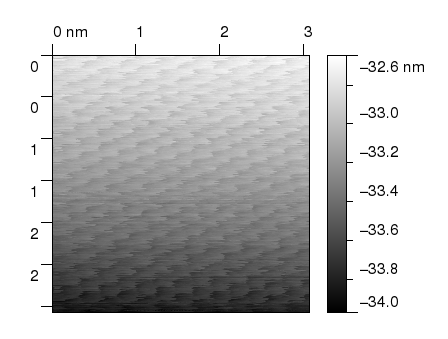
\includegraphics[width=\textwidth]{pics/fourier1}
    \end{subfigure}\qquad
    \begin{subfigure}[b]{\picwidth}
        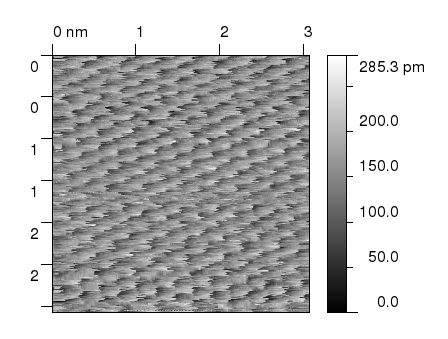
\includegraphics[width=\textwidth]{pics/fourier2}
    \end{subfigure}
    \caption{Links: Unbearbeitete Aufnahme aus Messung 13 (b), Rechts: Aufnahme mit
    subtrahiertem Hintergrund.}
    \label{fig:fourier12}
\end{figure}


Wir werden uns nun eine Mikroskopieaufnahme des Graphits vornehmen und anhand dessen zeigen,
wie mithilfe der statistischen Analyse Gittereigenschaften extrahieren können. 
Die Vorliegende Aufnahme ist noch unbearbeitet
und dementsprechend schwierig zu analysieren (siehe Abbildung~\ref{fig:fourier12}), da alle
Störungseinflüsse noch ungefiltert vorliegen.


Wir werden nun von mit einem lokalen Durchschnitt (\textit{moving average})
die Gradientenebene und den polynomiellen Hintergrund berechnen und diese von der Mikroskopie
subtrahieren (siehe Abbildung~\ref{fig:fourier12}). 
Abmessen einer Reihe und Abzählen ergibt
\begin{align*}
    d_h &= 0.24 \pm 0.02 nm \mbox{ (horizontale Axe)}\\
    d_v &= 0.18 \pm 0.02 nm \mbox{ (vertikale Axe)}
\end{align*}


\begin{figure}  
    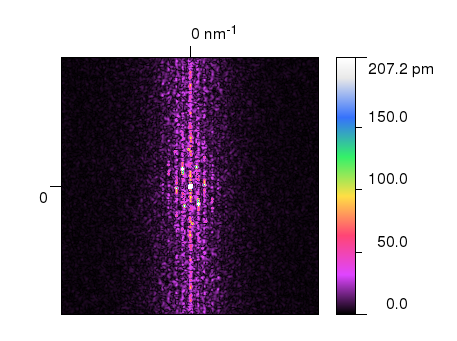
\includegraphics[width=10cm]{pics/fourier3}
  \caption{Leistungsspektrum der 2DFFT (2-dimensionale Fast-Fourier-Transformation) 
      mithilfe der Blackman Windowfunktion
  der Aufnahme. Hier sieht man deutlich das vertikal verschobene Sechseck in der Mitte,
  welches die Moden der Aufnahme darstellt.}
\label{fig:fourier3}
\end{figure}

Wir sehen also, dass der vertikale Abstand, verglichen mit dem Literaturwert ($0.246nm$), deutlich
geringer ist, dass also die gesamte Aufnahme in beide Richtungen zusammengezogen ist. 
Auch die horizontale Richtung ist im Mittel zu gering. Hierbei haben wir aber nur eine einzige
Linie analysiert, diese Methode ist allerdings sehr ungenau. 
Als nächstes können wir die Fouriertransformierte betrachten, dazu
berechnen wir die \textit{2DFFT} mithilfe der Windowfunktion \textit{Blackman} 
(siehe Abbildung~\ref{fig:fourier3}). Diese Fouriertransformationen kondensiert die Information
über die Moden der Aufnahme, allerdings sind auch alle Störungseinflüsse noch enthalten, trotzdem
ist schon deutlich das die erste Brillouinzone des reziproken Gitters in der Mitte zu erkennen
(Sechseck mit höherer Intensität). Die restliche Verteilung lässt sich auf viele Störeinflüsse
zurückführen. Um die periodischen Strukturen in der Aufnahme in Abbildung~\ref{fig:fourier12} zu
verstärken, wenden wir nun die 2DACF an. Es handelt sich dann nicht mehr um ein Feld im 
eigentlichen Ortsraum, bildet aber dieselben Periodizitäten, also in der gleichen Skala ab
(siehe Abbildung~\ref{fig:fourier4}). Die Fouriertransformation davon ist nun störungsbereinigt
und zeigt nur noch den reziproken Raum der Periodizität, die wir sehen wollen
(siehe Abbildung~\ref{fig:fourier5}). Die Fouriertransformierte bildet nun ab, was wir schon
im normalen Gitter gemessen haben, nämlich einen verlängerten vertikalen K-Vektor (analog
zu der verkürzten Achse im Ortsraum in vertikale Richtung), der nach dem Literaturwert 
erwartete K-Vektor wäre nämlich $4.065nm$. Dieser Einfluss auf die Skalierung
muss auf die Messung zurückgeführt werden. Über die Gründe können wir hier nur spekulieren und 
würde einer eingehenderen Analyse des Spektroskops bzw. der verwendeten Spitze bedürfen; 
ein möglicher Grund wäre beispielsweise, dass die Spitze nicht in allen Richtung gleichmäßig 
ausgerichtet war, sondern bei der vertikalen Richtung nach oben oder unten preferiert ausgerichtet
war und somit den Tunnelstrom verfälscht hat. Dazu müsste allerdings die Geometrie der Spitze 
analysiert werden, was im Rahmen unser Messungen nicht möglich war.
\begin{SCfigure}
    \caption{2DACF der Aufnahme (Abbildung~\ref{fig:fourier12}) mit
    subtrahiertem Hintergrund. }
    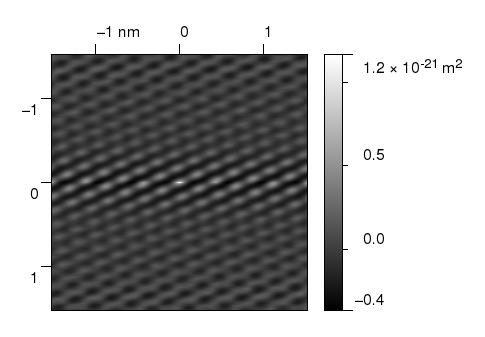
\includegraphics[width=0.7 \textwidth]{pics/fourier4}
    \label{fig:fourier4}
\end{SCfigure}
\begin{SCfigure}
    \caption{2DFFT der autokorrelierten Aufnahme.}
    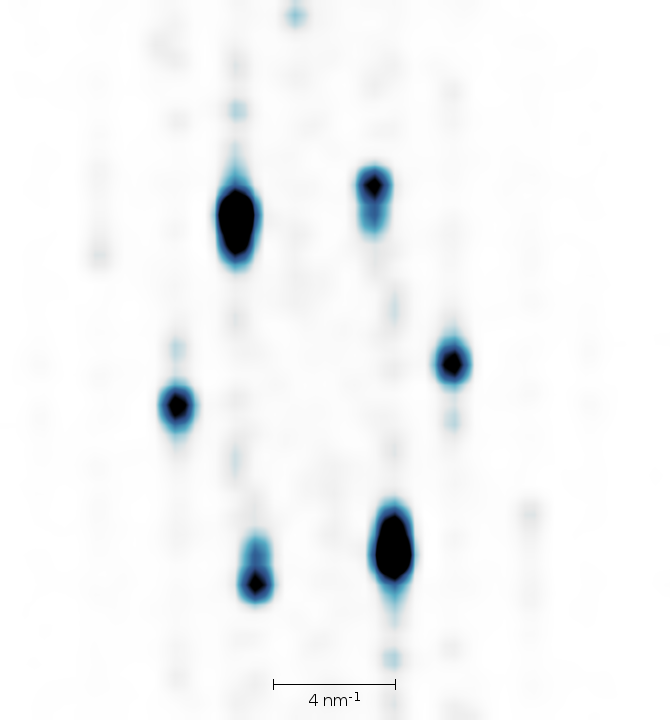
\includegraphics[width=0.7 \textwidth ]{pics/fourier5}
    \label{fig:fourier5}
\end{SCfigure}



\clearpage
